\documentclass[UTF8]{ctexart}
\usepackage{geometry, CJKutf8}
\geometry{margin=1.5cm, vmargin={0pt,1cm}}
\setlength{\topmargin}{-1cm}
\setlength{\paperheight}{29.7cm}
\setlength{\textheight}{25.3cm}

% useful packages.
\usepackage{amsfonts}
\usepackage{amsmath}
\usepackage{amssymb}
\usepackage{amsthm}
\usepackage{enumerate}
\usepackage{graphicx}
\usepackage{multicol}
\usepackage{fancyhdr}
\usepackage{layout}
\usepackage{listings}
\usepackage{float, caption}

\lstset{
	basicstyle=\ttfamily, basewidth=0.5em
}

% some common command
\newcommand{\dif}{\mathrm{d}}
\newcommand{\avg}[1]{\left\langle #1 \right\rangle}
\newcommand{\difFrac}[2]{\frac{\dif #1}{\dif #2}}
\newcommand{\pdfFrac}[2]{\frac{\partial #1}{\partial #2}}
\newcommand{\OFL}{\mathrm{OFL}}
\newcommand{\UFL}{\mathrm{UFL}}
\newcommand{\fl}{\mathrm{fl}}
\newcommand{\op}{\odot}
\newcommand{\Eabs}{E_{\mathrm{abs}}}
\newcommand{\Erel}{E_{\mathrm{rel}}}

\begin{document}
	
	\pagestyle{fancy}
	\fancyhead{}
	\lhead{王琰博, 3220105837}
	\chead{数据结构与算法第四次作业}
	\rhead{Oct.16th, 2024}
	
	\section{测试程序的设计思路}
	
	根据提示首先编写出detachMin函数,大体思路与之前的findMin类似,通过递归找到最小节点,再将其用另一变量记录并返回后删除该节点,即返回该节点右侧的分支,若右侧无分支则返回空指针。
		
		\begin{figure}[H] %H为当前位置,!htb为忽略美学标准,htbp为浮动图形
			\centering %图片居中
			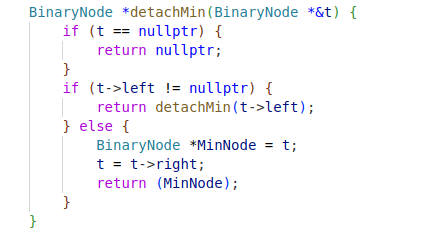
\includegraphics[width=0.7\textwidth]{fig1} %插入图片,[]中设置图片大小,{}中是图片文件名
			\caption{detachMin} %最终文档中希望显示的图片标题
		\end{figure}
		
	
	
	接下来用指针实现remove函数。只需要利用上面的detachMin函数,在删除具有左右分支节点时搜寻其右侧分支的最小值并将其记录再删除,并且将需要删除的节点替换为该值,同时将删除节点的左右分支连接至该节点,即可实现。
		
		\begin{figure}[H] %H为当前位置,!htb为忽略美学标准,htbp为浮动图形
			\centering %图片居中
			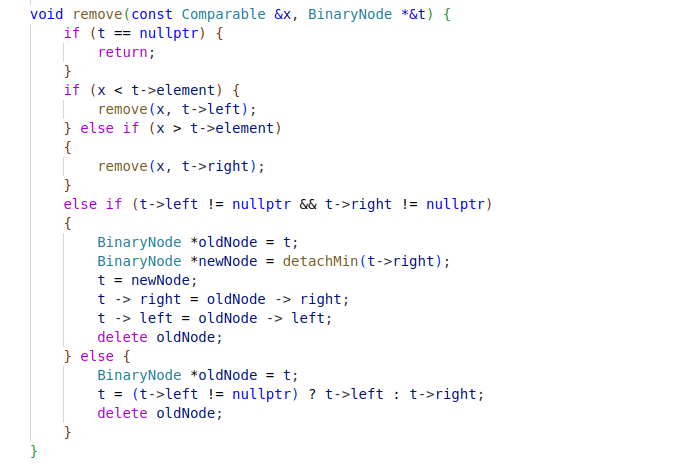
\includegraphics[width=0.7\textwidth]{fig2} %插入图片,[]中设置图片大小,{}中是图片文件名
			\caption{remove} %最终文档中希望显示的图片标题
		\end{figure}
		
	
	
	测试程序的设计主要分别进行了对无分支节点的删除,对有一分支节点的删除,对有两分支节点的删除以及对根节点的删除。

		\begin{figure}[H] %H为当前位置,!htb为忽略美学标准,htbp为浮动图形
			\centering %图片居中
			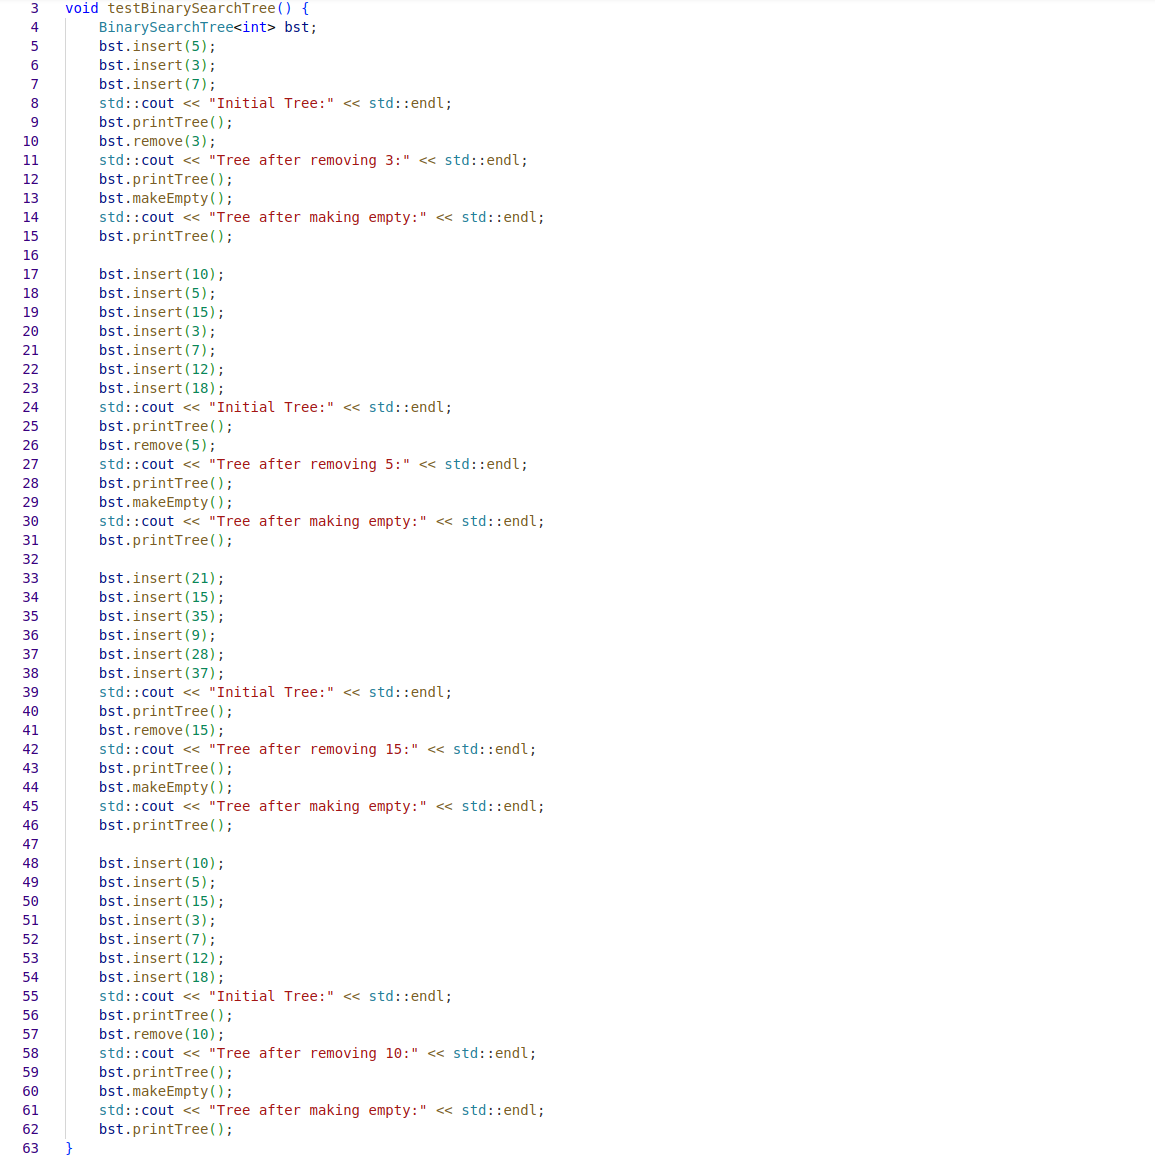
\includegraphics[width=0.7\textwidth]{fig3} %插入图片,[]中设置图片大小,{}中是图片文件名
			\caption{test\_DST} %最终文档中希望显示的图片标题
		\end{figure}
		
	\section{测试的结果}
	
	测试结果一切正常。
	
	输出为: 
		
		\begin{figure}[H] %H为当前位置,!htb为忽略美学标准,htbp为浮动图形
			\centering %图片居中
			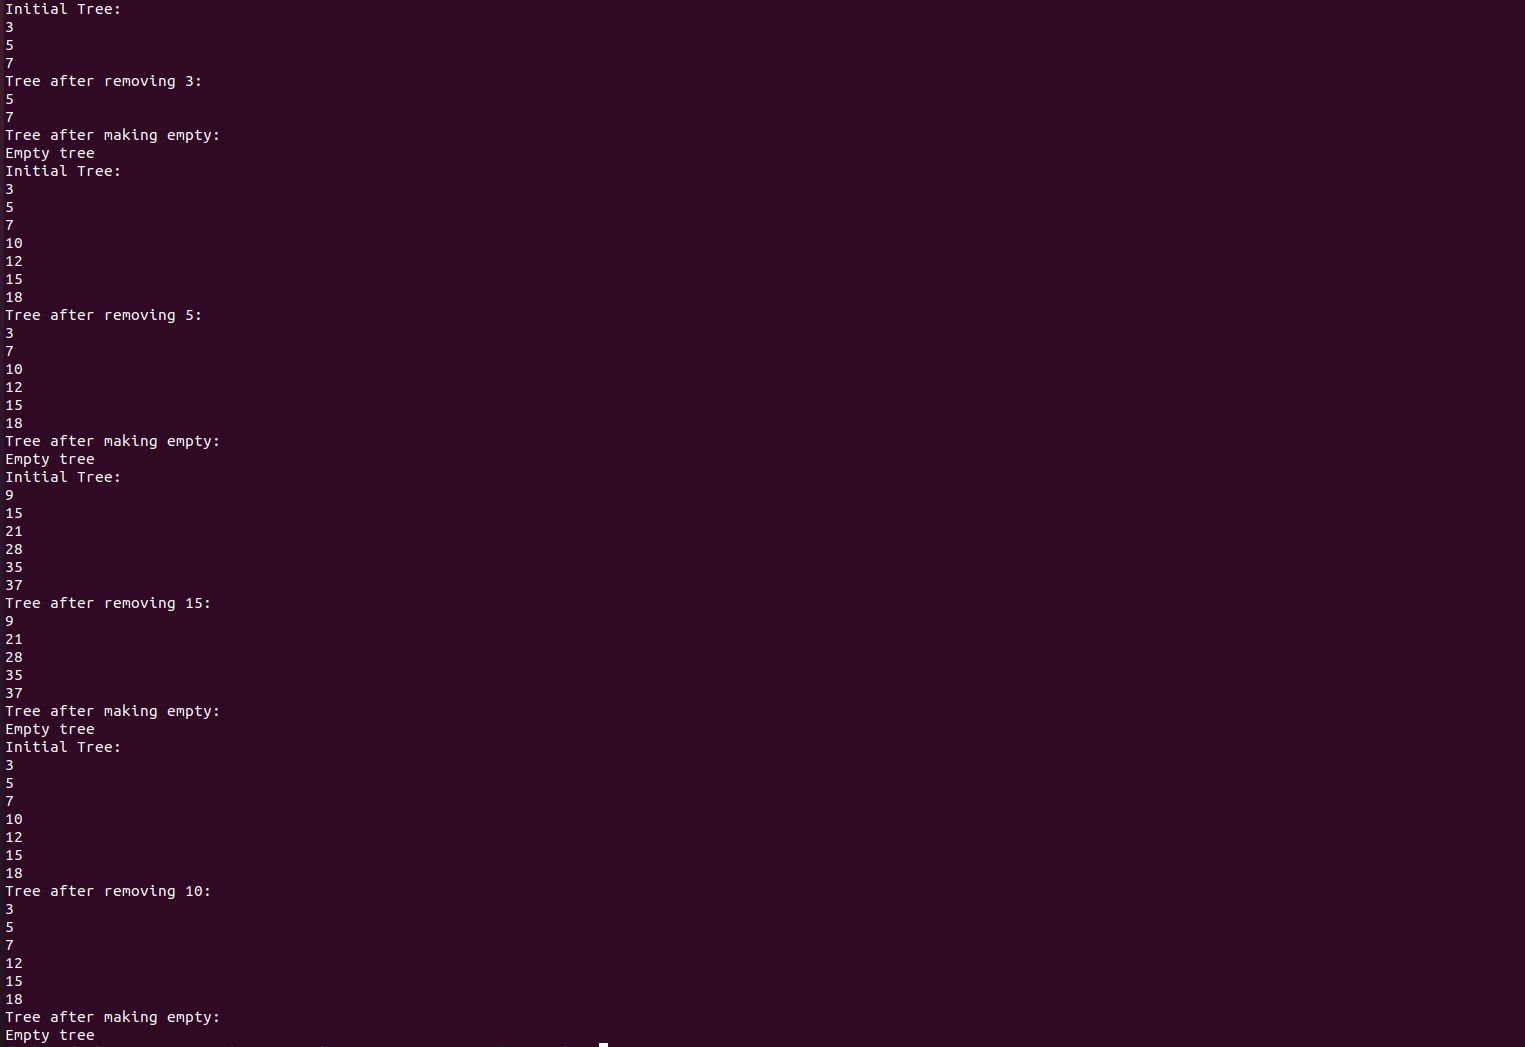
\includegraphics[width=0.7\textwidth]{fig4} %插入图片,[]中设置图片大小,{}中是图片文件名
			\caption{output} %最终文档中希望显示的图片标题
			\label{Fig.main2} %用于文内引用的标签
		\end{figure}
		
	
	\section{bug报告}
	
	一切正常。
	
	%%% Local Variables: 
	%%% mode: latex
	%%% TeX-master: t
	%%% End: 
\end{document}